\documentclass[a4paper, 12pt]{article}

\usepackage{cmap} % поиск в PDF
\usepackage[english, russian]{babel} % локализация и переносы
\parskip=3pt % дополнительное расстояние между абзацами
\usepackage{graphicx} % вставка рисунков
\usepackage{lastpage}
\usepackage{rotating}
%\usepackage{minted} % красивый код
\usepackage{verbatim}
\usepackage{multirow} % Слияние строк в таблице
\usepackage{caption}
\usepackage{amsfonts, amssymb, amsthm, mathtools, amsmath} % AMS
\usepackage{array} % Дополнительная работа с таблицами
\usepackage{multicol}

%%% Цветной текст

\usepackage[usenames]{color}
\usepackage{colortbl}

%% Поля

\usepackage{geometry} 
\geometry{left=2cm}
\geometry{right=2cm}
\geometry{top=2cm}
\geometry{bottom=2cm}

%%% Гиперссылки

\usepackage[unicode]{hyperref}
\usepackage{xcolor}
\definecolor{urlcolor}{HTML}{4682B4} % цвет гиперссылок
\definecolor{linkcolor}{HTML}{4682B4} % цвет ссылок
\definecolor{citecolor}{HTML}{4682B4} % цвет библиоссылок
\hypersetup{pdfstartview=FitH,  linkcolor=linkcolor,urlcolor=urlcolor, citecolor=citecolor, colorlinks=true}

%% Немного дизайна

\definecolor{lb}{rgb}{0.8,0.85,1}
\renewcommand{\labelitemi}{$\diamond$}


\begin{document}

\thispagestyle{empty}
\begin{center}
	\textbf{ПРАВИТЕЛЬСТВО РОССИЙСКОЙ ФЕДЕРАЦИИ}\\
	\vspace{3ex}
	\textbf{Федеральное государственное автономное\\ образовательное учреждение высшего образования}
	
	\vspace{3ex}
	
	\textbf{Национальный исследовательский университет \\ <<Высшая школа экономики>>}
	
	\vspace{10ex}
	\begin{flushright}
		Факультет экономических наук\\
		Образовательная программа <<Экономика>>
	\end{flushright}
\end{center}
\vspace{12ex}

\begin{center}
	{\textbf{КУРСОВАЯ РАБОТА
	}}
	\vspace{1ex}
	
	<<Новая тема>>
\end{center}
\vspace{4ex}
\begin{flushright}
	\noindent
	Студентка группы БЭК171\\Махнева Елизавета Александровна\\
	\vspace{13ex}
	Научный руководитель:\\
	Соколов Евгений Андреевич
	
\end{flushright}	

\vfill

\begin{center}
	Москва 2020
	
\end{center}
\newpage
	\tableofcontents
	\newpage
	
	\section{Введение}
	Во введении я хочу сказать про то что существует интерпретируемые и нет модели. Про то что нам хотелось бы интерпретировать и привести аргументы за (как минимум те 3 из презенташки). Наверное стоит объединить с блоком интерпретации, так как здесь особо больше нечего писать (если только много не получится), а воду лить не хочется

1. Интерпретируемые и нет модели. Желательно показать примеры, почему не интерпретируются.
2. Интерпретация нужна! Потому что...
3. Плюсы интерпретации и небольшие минусы
4. Что и как хотелось бы интерпретировать. Основы интерпретации -- какой она должна быть
5. Кратко перечислить методы, сказать какие они бывают
	\newpage
	
	\section{Интерпретация - подумать над названием}
	\subsection{Зачем она нужна}
	Блин, это же было во введении. Да, точно надо объединять	
	\subsection{Что можно интерпретировать}
	\input{chapters/2_2inter.tex}
	\subsection{Методы}
	\input{chapters/2_3inter.tex}
	\newpage
	
	\section{Методы и их принципы}
	\subsection{PDP + реализация}
	\textbf{PDP (Partial Dependence Plot, график частичной зависимости)} -- график, который показывает зависимость прогноза модели от значения отдельного признака. С его помощью мы можем понять, как некоторый признак влияет на предсказание. Данный график можно изобразить для двух либо трех признаков из имеющихся.

\subsubsection{Идея}
Визуализация -- это отличный способ интерпретации. Если мы хотим понять, как признаки влияют на результат, можно посмотреть, как меняется прогноз от изменения одного признака при прочих равных. В идеальной ситуации мы бы построили график зависимости результата от всех признаков и меняли бы только один. Однако мы сталкиваемся с проблемой: если признаков больше двух, построить график не получится. Поэтому чтобы сохранить возможность визуализации, можно анализировать зависимость результата от одного признака без учета влияния остальных, построив график зависимости от одного признака. Аналогично можно изучать влияние одновременно двух признаков, построив трехмерный график.

<Пример 2мерного и 3мерного графиков>
	\subsection{LIME + реализация}
	LIME (Local Interpretable Model-Agnostic Explanations) -- метод, показывающий вклад признаков в отдельное предсказание, работающий с любой моделью.
% нужен ли перевод

\subsubsection{Идея}
Результаты некоторых моделей легко интерпретировать. Например, в линейной регрессии можно посмотреть на веса. Они показывают, насколько изменится предсказание при изменении признаков. Так для каждого конкретного предсказания можно понять, почему модель выдала именно такой результат -- виден непосредственный вклад каждого признака.

Но не все модели легко интерпретировать. Например, некоторые архитектуры нейронных сетей. Они зачастую значительно превосходят линейные модели, но при этом сама структура модели представляет собой <<черный ящик>> -- непонятно, как именно модель сформировала предсказание, какие признаки сильнее повлияли на решение нейронной сети.

Идея состоит в том, чтобы перенести свойство интерпретируемости простых моделей на более сложные. Мы можем обучить интерпретируемую модель по выборке, где ответами являются предсказания сложной модели. В процессе обучения модель анализирует зависимости непосредственно между признаками и предсказаниями сложной модели. Тогда мы сможем интерпретировать результаты простой модели, которые являются аппроксимацией предсказаний сложной.\\[2mm]
\begin{minipage}{0.57\linewidth}
\indent Возникает проблема: сложная модель выявляет зависимости, которые, например, линейная модель может не уловить. Идея данного метода заключается в том, чтобы обучать более простую модель в некоторой окрестности исследуемого объекта, предполагая что на очень локальном уровне нет сложных зависимостей. Например, дифференцируемые функции можно линеаризовать в окрестности заданной точки -- можно использовать линейную модель на локальном уровне.
\end{minipage}
\hspace{5mm}
\begin{minipage}{0.35\linewidth}
	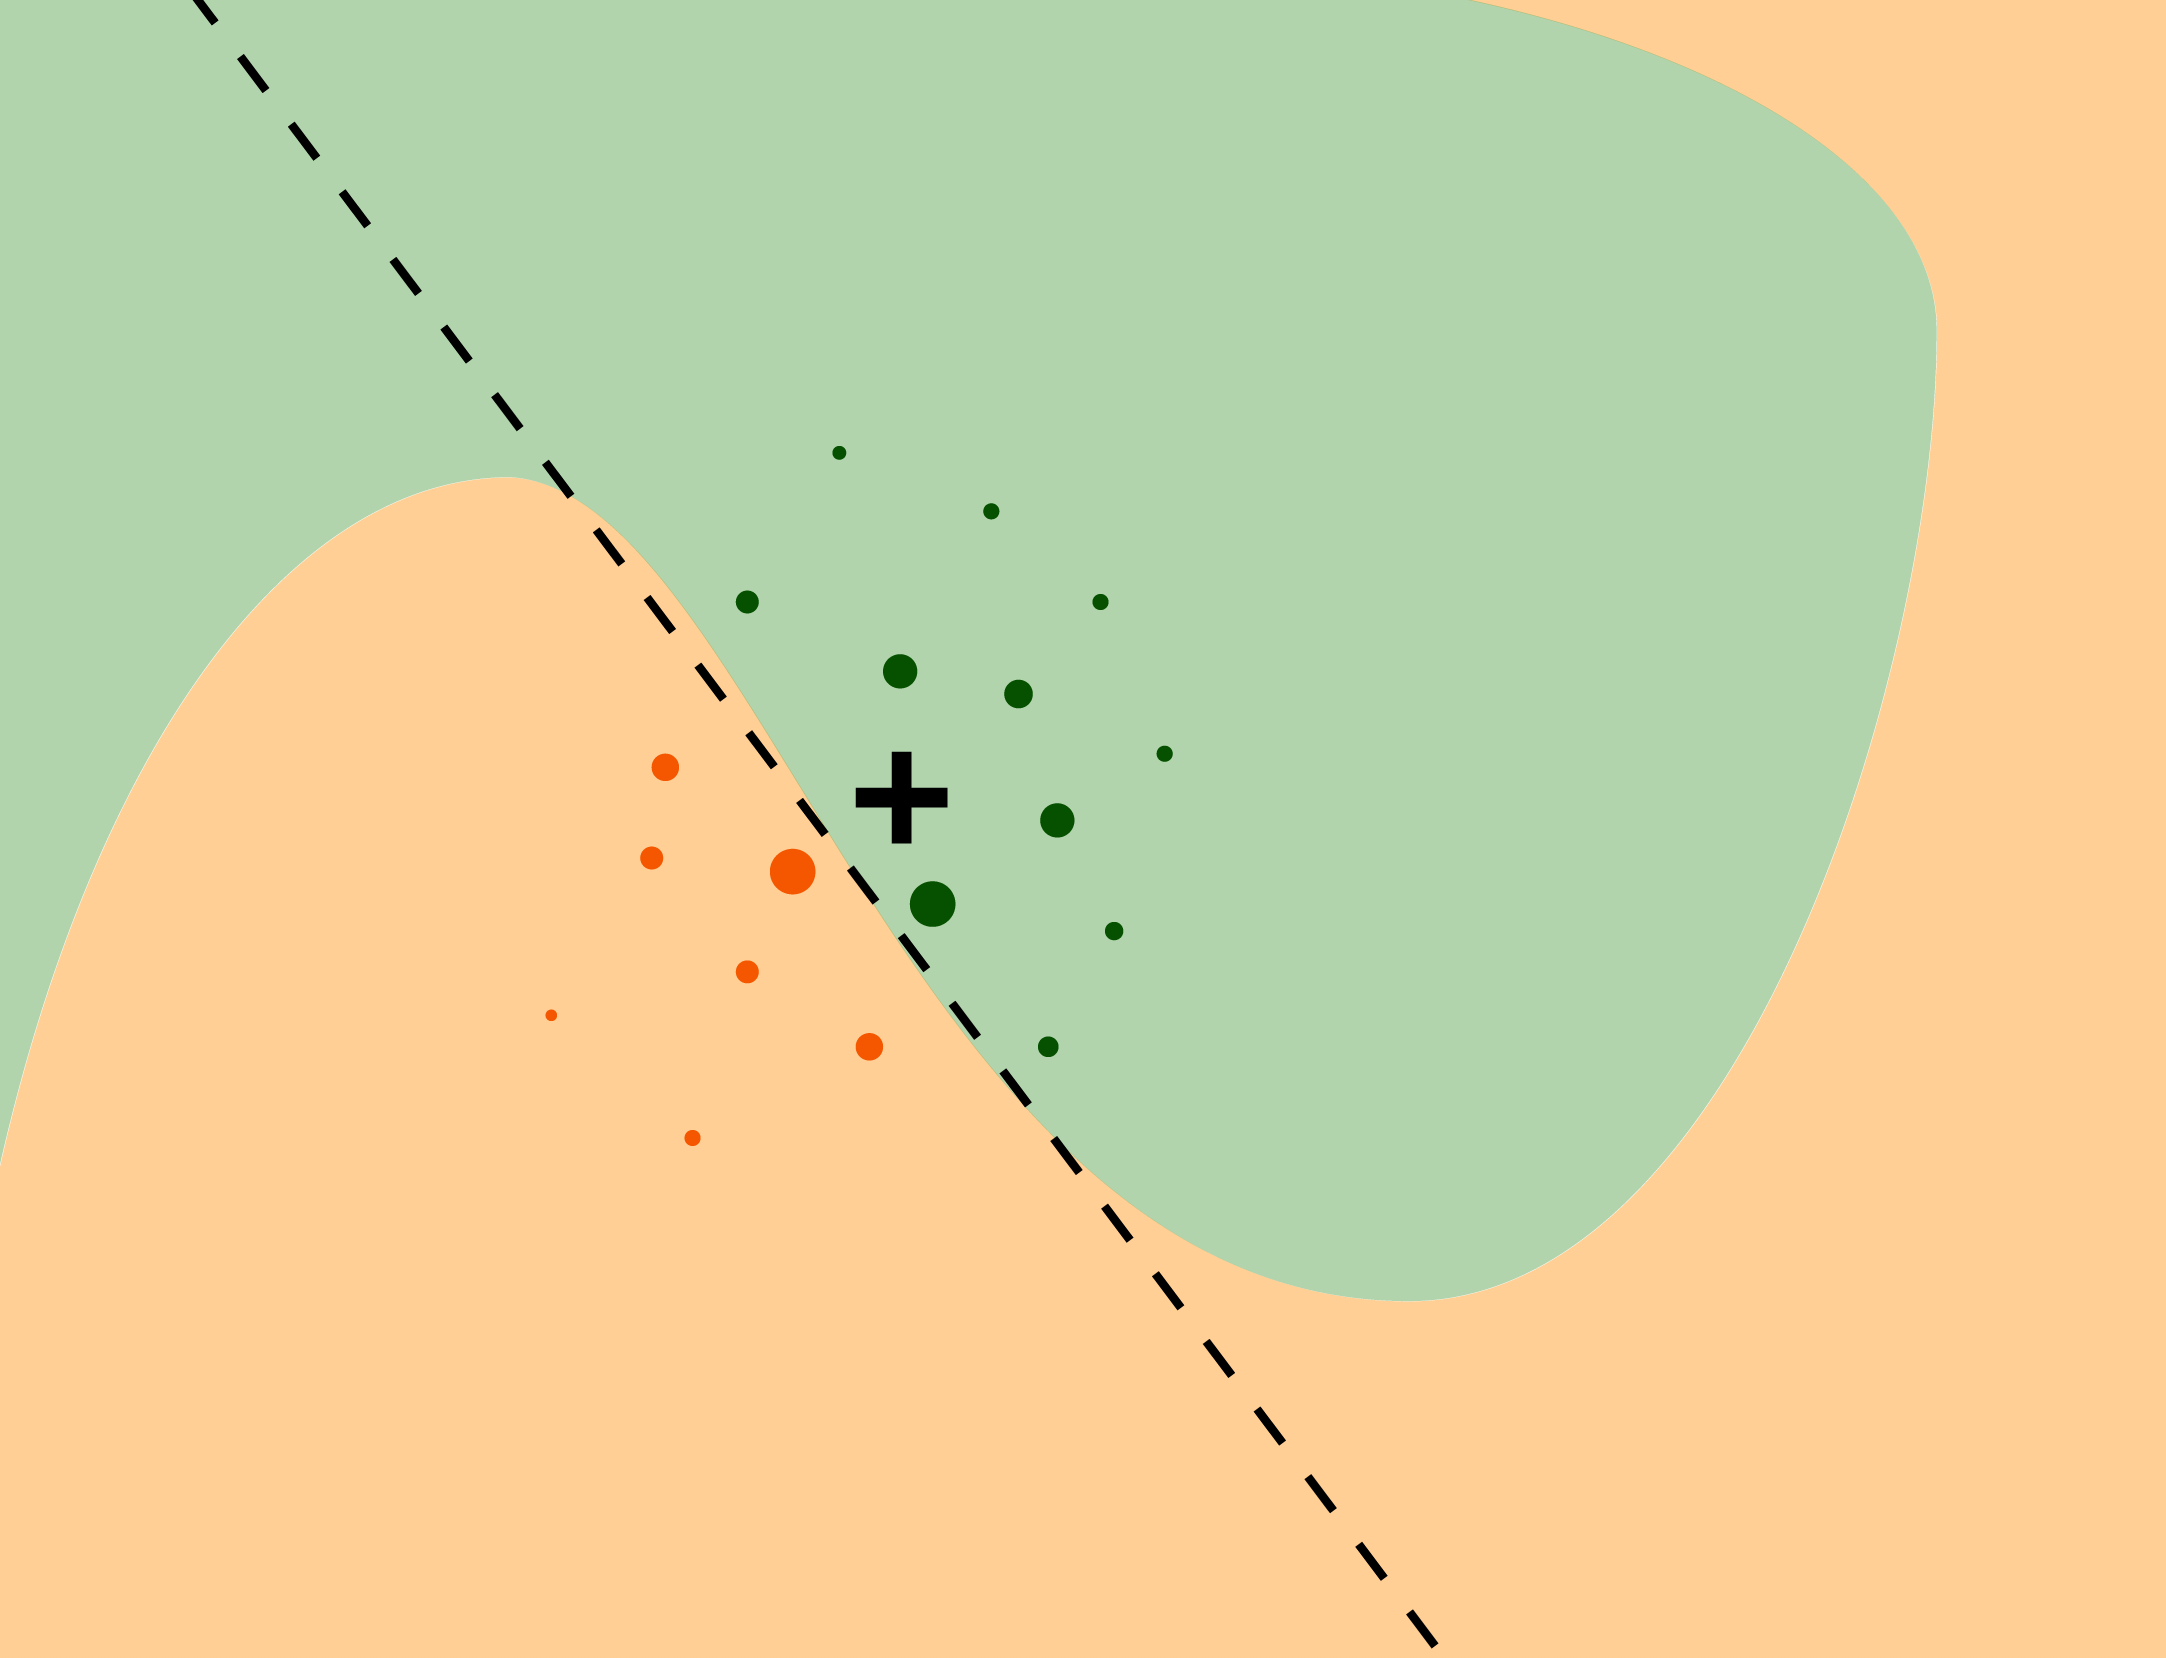
\includegraphics[width=6.5cm, height=5cm]{pics/lime4.png}
\end{minipage}

\underline{Пример LIME для табличных данных}
\vspace{-3mm}

\begin{figure}[h]
	\centering{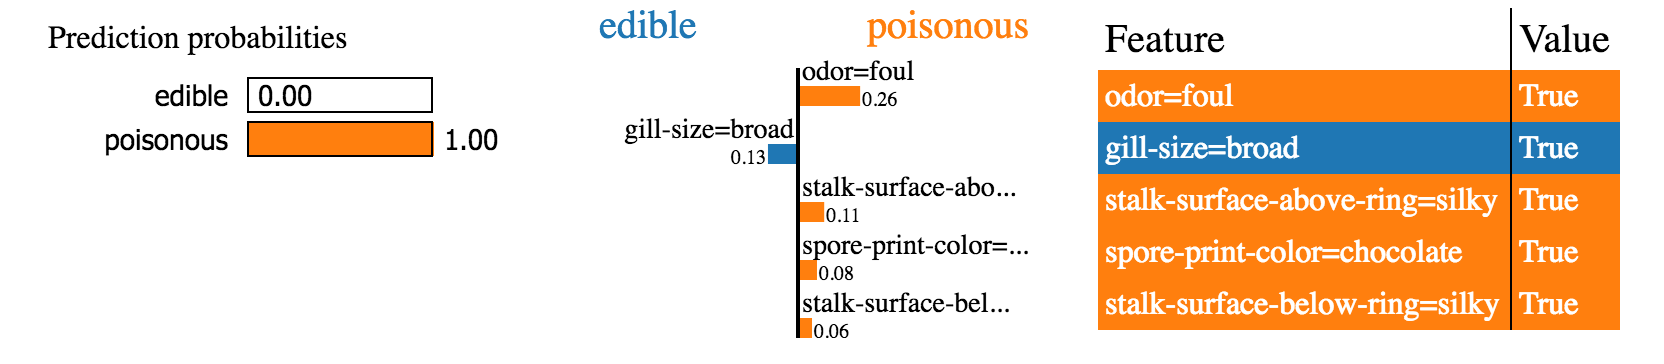
\includegraphics[width=\linewidth]{pics/lime1.png}}
\end{figure}

В данном случае решалась задача бинарной классификации. LIME вывел пять самых значимых признаков и показал, каким образом они повлияли на предсказание. Обученная модель показала, что исследуемый объект принадлежит к классу <<poisonous>>. И по анализу LIME понятно почему: только один признак из выведенных увеличил вероятность принадлежности объекта к классу <<edible>> и только на $0.13$. В то же время оставшиеся четыре признака повлияли на вероятность объекта быть <<poisonous>>, причем суммарно увеличив вероятность на $0.51$. Данная интерпретация позволяет понять, адекватна ли модель, которую мы получили, действительно ли релевантные признаки оказались значимыми.

\underline{Пример LIME для текстов}
\vspace{-3mm}

\begin{figure}[h]
	\centering{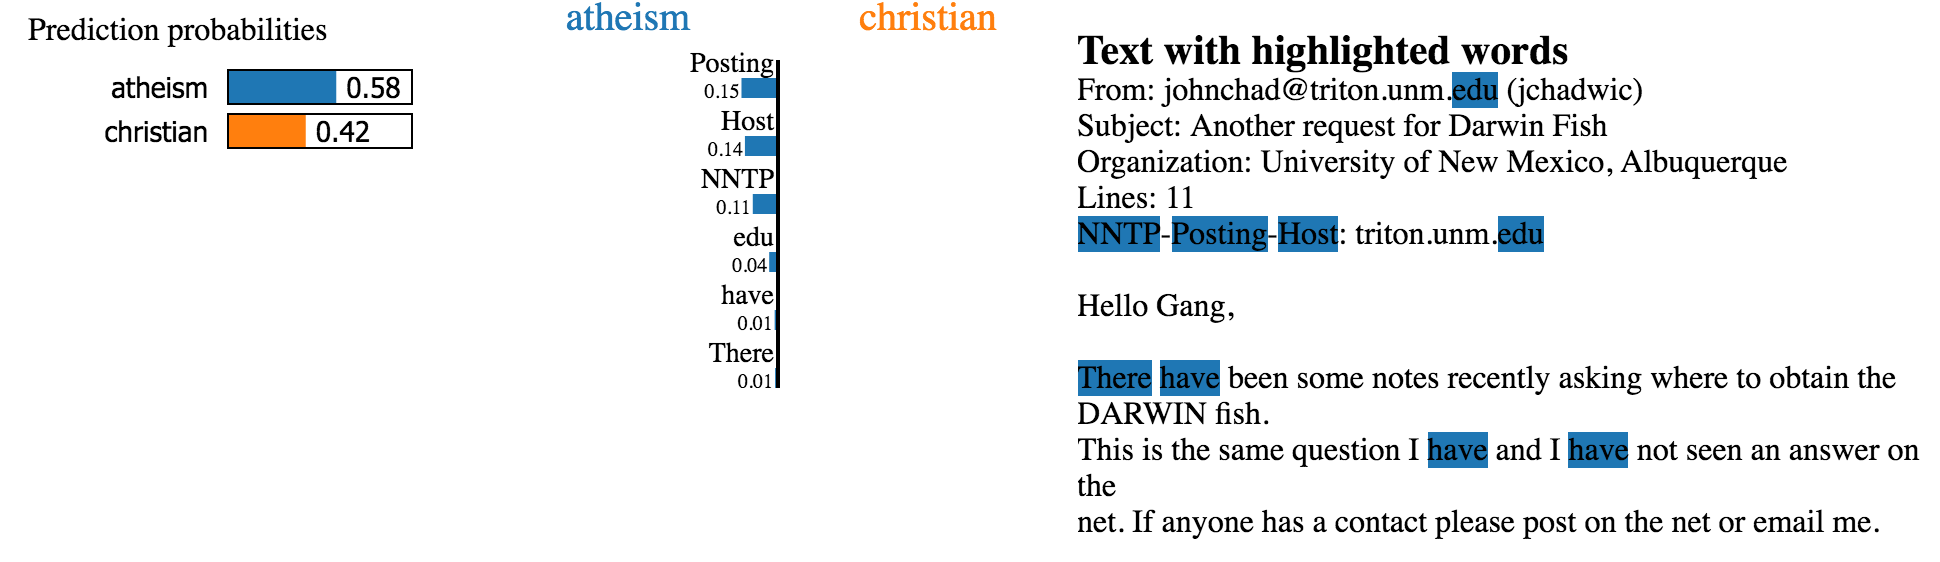
\includegraphics[width=\linewidth]{pics/lime2.png}}
\end{figure}

\underline{Пример LIME для картинок}
\vspace{-3mm}

\begin{figure}[h]
	\centering{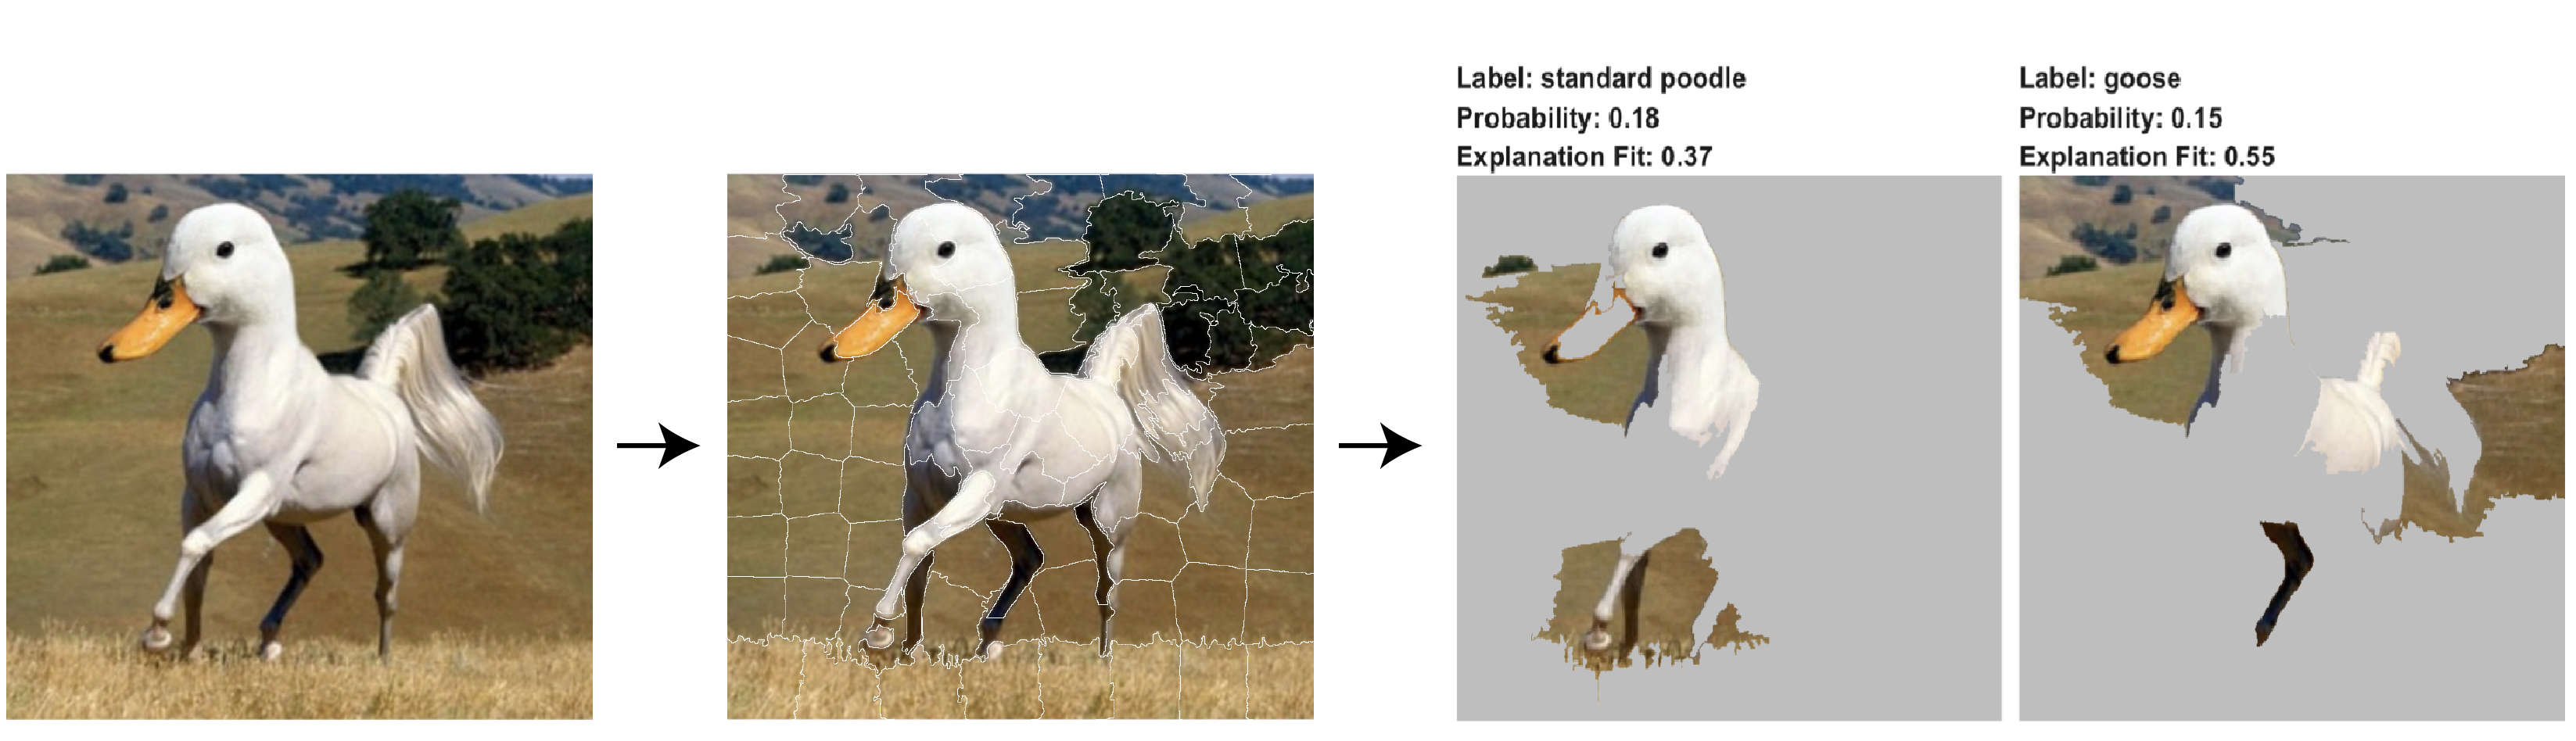
\includegraphics[width=\linewidth]{pics/lime3.png}}
\end{figure}

% почему не вытаскивать из самих моделей?
	\subsection{SHAP + реализация}
	SHAP (SHapley Additive exPlanations) -- метод, оценивающий вклад признаков в предсказания модели на основе значений Шэпли.

\subsubsection{Идея}
Предсказание модели формируется на основе признаков. Если мы хотим узнать влияние отдельного признака, мы можем построить предсказание модели с ним и без него и затем посмотреть, как меняется результат. % почему реально не убирать насовсем?
Но модель может быть слишком сложной, чтобы мы могли оценить влияние предиктора по одному объекту, регулируя один признак при фиксированных остальных. % а корректно ли занулять его, это ведь тоже какое-то значение
% помнить про то, что у shapley values есть свой раздел
Правильнее рассмотреть все возможные комбинации признаков: их разные значения, наличие/отсутствие, чтобы понять, как в каждом из перечисленных случаев добавление и исключение признака влияет на предсказание.

Рассматривая влияние в каждом конкретном случае, мы получаем огромное количество предельных эффектов, что тяжело интерпретируется. Поэтому можно рассмотреть, какой в среднем эффект оказывает включение признака в модель. Тогда мы получим средневзвешенную оценку вклада отдельного признака в предсказание, что позволит проинтерпретировать результат работы модели.
% Подумать, почему они сравнивают результат со средним кроме как кроме того что нужна всего одна модель и теряется точность

Однако для такого способа нужно обучить количество моделей, равное количеству всех комбинаций признаков -- которое растет экспоненциально с увеличением количества признаков. Вместо этого мы можем аппроксимировать разницу между предсказаниями разных моделей разницей между предсказанием и ожидаемым предсказанием. % дописать идею

% мб метод SHAP вносит еще какие-то идеи, но пока что так

\subsubsection{Значения Шэпли (Shapley values)}
Для упрощения расчетов мы не будем рассматривать разные значения предикторов, а бинаризуем их представление, обозначив за <<1>> наличие предиктора и за <<0>> его отсутствие.
% наверняка можно как-то умнее упрощать признаки
% в чем отличие SHAP?
Тогда у нас есть некоторое ограниченное количество возможных комбинаций признаков. Пусть $S$ -- множество ненулевых признаков, в которое не входит исследуемый $i$-ый признак. Чтобы найти разницу предсказаний для признаков из $S$ и из $S \cup \{i\}$, куда входит $i$-ый признак, нам нужно обучить две модели, $f_S$ и $f_{S \cup \{i\}}$, соответственно. Тогда для объекта $x$ мы получим:
\[
f_{S \cup \{i\}}(x_{S \cup \{i\}}) - f_S(x_S),
\]

Как отмечалось ранее, значения данного выражения могут меняться при разных комбинациях признаков, поэтому мы усредним ее для всех возможных случаев. Считая, что $F$ -- множество всех признаков, получим итоговое выражение для $i$-го признака:
\[
\phi_i = \frac{1}{|F|} \sum\limits_{S \subseteq F \backslash \{i\}}
\begin{pmatrix}
|F| - 1 \\
|S|
\end{pmatrix}^{-1}
(f_{S \cup \{i\}}(x_{S \cup \{i\}}) - f_S(x_S)),
\]
где $|F|$ -- количество элементов в множестве $F$, $|S|$ -- в множестве $S$.

Коэффициент:
\[
\ds \begin{pmatrix}
|F| - 1 \\
|S|
\end{pmatrix} = \frac{(|F|-1)!}{|S|! \cdot (|F| - |S| - 1)!}
\]
равен количеству всех возможных комбинаций признаков без учета исследуемого. Поделив на него, а также на количество признаков получаем среднее значение вклада признака. % а зачем делить на колво признаков

Данный коэффициент также можно интерпретировать как вес комбинации при расчете среднего. Биномиальный коэффициент, равный количеству комбинаций, для одного или $|F|-1$ признаков меньше, чем для любого другого числа признаков. Соответственно, при делении на коэффициент мы получаем большее значение, который указывает на больший вес подобных комбинаций. Это имеет смысл, так как больше информации мы получаем, рассматривая влияние признаков по отдельности: либо оставляя только его, либо исключая все кроме него. С увеличением количества признаков в $S$ вес комбинации убывает.

Таким образом, мы получили величину, показывающую, какой в среднем вклад вносит конкретный признак в предсказание. Данное значение пришло из теории игр и носит название значение Шэпли (Shapley value). Они показывают, какой вклад внес в общий выигрыш отдельный игрок при кооперации. В нашей задаче мы рассматриваем предсказание модели как выигрыш, а признаки как игроков.
	\newpage

	\section{Примеры}
	\subsection{Первый прикольный пример}
	\input{chapters/4_1ex.tex}
	\subsection{Второй прикольный пример}
	\input{chapters/4_2ex.tex}
	\newpage

	\section{Данные и модели}
	Рассмотрим описанные методы на конкретной задаче. Построим относительно сложную модель (градиентный бустинг) для бинарной классификации объектов. Помимо этого построим несколько интерпретируемых моделей (логистическая регрессия, решающее дерево), чтобы сравнить значимость, которую они придают предикторам, с анализом методов интерпретации.
	\subsection{Данные}
	Для анализа был выбран датасет, содержащий информацию о клиентах разных отелей за 2015-2017 года. Задача: предсказать, отменит ли клиент бронь. Датасет был предварительно обработан:
\begin{itemize}
	\item Удалены переменные company (много пропусков), reservation status, reservation status date (данная информация обычно бывает известна уже после отмены либо отъезда гостя)
	\item Приведены к числовому виду порядковые переменные meal, deposit type, arrival date month
	\item Удалены строки с пропущенными значениями -- таких строк было немного и в них была пропущена важная информация
\end{itemize}

Отдельн стоит отметить, что категориальные переменные reserved room type, assigned room type, hotel, country, market segment, distribution channel, customer type не были приведены к числовому виду, так как далее (спойлер) будет использоваться модель CatBoost, которая самостоятельно обрабатывает такие признаки.
	\subsection{Модели}
	Для анализа описанных методов я выбрала следующие модели: CatBoost (сложная модель), логистическая регрессия (простая интерпретируемая модель) и решающее дерево (простая интерпретируемая модель)

\paragraph{CatBoost.}
В первую очередь мне необходимо установить и импортировать данную библиотеку

$\verb|pip install catboost|$

$\verb|from catboost import CatBoostClassifier|$

\paragraph{LogisticRegression и DecisionTreeClassifier.}
Я буду использовать реализации данных моделей в $\verb|sklearn|$:

$\verb|from sklearn.linear_model import LogisticRegression|$

$\verb|from sklearn.tree import DecisionTreeClassifier|$

Обе модели имеют встроенные методы для извлечения важности признаков, поэтому будет легко интерпретировать их предсказания.
% здесь заметка про важность признаков у деревьев
	\subsection{Попытка интерпретации}
	Модель достигла неплохого качества в задаче классификации: ROC-AUC=0.9, accuracy=0.82. Попробуем интерпретировать ее результаты.

Нулевой способ это встроенный метод XGBoost, показывающий важность признаков при предсказании. Посмотрим на первые 5 самых важных признаков. Данная величина может быть расчитана тремя способами: <<weight>>, <<gain>>, <<cover>>. Первый показывает, сколько раз признак появляется в дереве:

\begin{figure}[h]
	\centering{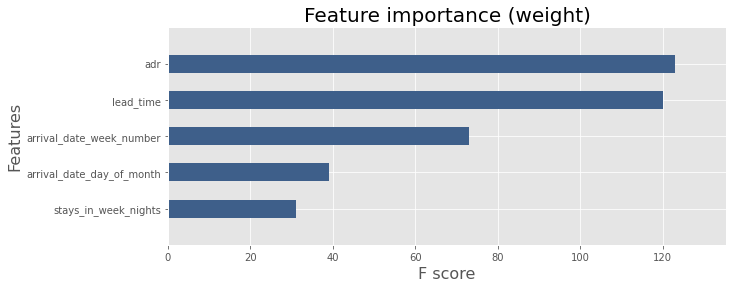
\includegraphics[width=0.85\linewidth]{pics/imp1.png}}
\end{figure}

Второй -- на сколько в среднем уменьшалась ошибка при использовании данного признака:

\begin{figure}[h]
	\centering{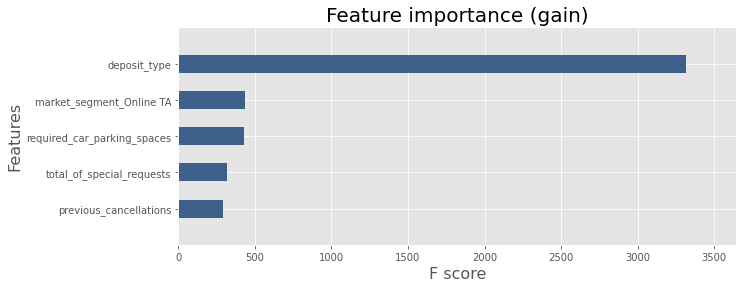
\includegraphics[width=0.85\linewidth]{pics/imp2.png}}
\end{figure}

И последний -- какое количество объектов выборки задействовало узлы с заданным признаком:

\begin{figure}[h]
	\centering{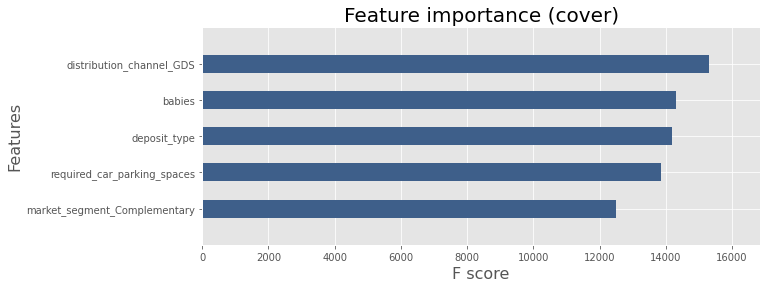
\includegraphics[width=0.85\linewidth]{pics/imp3.png}}
\end{figure}

Теперь перейдем к описанным ранее методам. Первый -- PDP. Возьмем признаки, которые сам XGBoost посчитал наиболее важными: первые два из weight (adr, lead\_time), первый из gain (deposit\_type) и первый из cover (distribution\_channel\_GDS) -- они с отрывом вырываются в лидеры.

И также возьмем признаки, которые XGBoost счел самыми незначительными: последний из weight (distribution\_channel\_GDS, забавно -- в тренировочной выборке всего 145 объектов, которым соответствует GDS. Судя по всему данный признак встречается 1-2 раза в узлах деревьев, но при этом он отсекает очень много объектов, из-за чего cover считает его важным), последние два из gain (customer\_type\_group, market\_segment\_Direct) и последний из cover (market\_segment\_Offline TA/TO).

Построим для них PDP. % на непрерывные как-то поадекватнее смотреть

\begin{tabular}{c|c}
	\arrayrulecolor[rgb]{0.8,0.85,1}
	\includegraphics*[width = 0.47\textwidth]{pics/mypdp1.png} & \includegraphics*[width = 0.47\textwidth]{pics/mypdp2.png}\\
	\hline
%	\includegraphics*[width = 0.5\textwidth]{mypdp3.png} & \includegraphics*[width = 0.5\textwidth]{mypdp4.png}}\\
%	\hline
%	\includegraphics*[width = 0.5\textwidth]{mypdp5.png} & \includegraphics*[width = 0.5\textwidth]{mypdp6.png}\\
%	\hline
%	\includegraphics*[width = 0.5\textwidth]{mypdp7.png} & \includegraphics*[width = 0.5\textwidth]{mypdp8.png}\\
\end{tabular}\\[2mm]
	\newpage
	
	\section{Анализ результатов}
	ы
	\newpage
	
	\section{Заключение}
	Таким образом, существующие методы интерпретации моделей машинного обучения показывают неплохие результаты. Безусловно, они имеют свои недостатки, но несмотря на это они справляются со своей задачей и с некоторой погрешностью объясняют работу сложных моделей.
	\newpage
	
	\begin{thebibliography}{99}
		\bibitem{basis}
		\href{https://christophm.github.io/interpretable-ml-book/}{Interpretable Machine Learning | Christoph Molnar | Christoph Molnar | 2020 | all pages}
	\end{thebibliography}
\end{document}